%\documentclass[twocolumn]{article}
\documentclass{report}

\usepackage{url}
\usepackage{indentfirst}
\usepackage{float}
\usepackage{listings} % Include the listings-package
\usepackage{mdframed}
\usepackage[numbers,sort]{natbib}
%\usepackage{titlesec} % Needed to support sub-subsections
%\usepackage[english]{babel} % Need for text wrap in table.
\usepackage{array} % Needed for centering in the table
\usepackage{graphicx}

% Defines the table of contents depth and the subsection numbering depth
\setcounter{secnumdepth}{5}
\setcounter{tocdepth}{5}

\title{\emph{HamSkill}: Run Haskell Anywhere \\
with ANTLR and Scala\\[1in]
	   CS252 Project Final Report}

\author{
  Zayd Hammoudeh \\
  (zayd.hammoudeh@sjsu.edu)
  }


\newcommand{\myparagraph}[1]{\paragraph{#1}\mbox{}\\}

% Skip lines after each paragraph.
\setlength\parskip{\baselineskip}

\begin{document}

\maketitle

\pagenumbering{roman}

\tableofcontents{\protect\newpage}

\listoffigures
\newpage
 
\pagenumbering{arabic}

\renewcommand\thesection{\arabic{section}}

\section{Running in the Java Virtual Machine}\label{sec:jvm}

C/C++ are two of the most commonly used languages when the goal is maximum performance.  However, C/C++'s ``write once, compile anywhere" paradigm limits its portability.  In contrast, the near ubiquity of the Java Virtual Machine (JVM) allows Java to be ``write once, run anywhere."  

On many occasions, developers have leveraged the JVM's ``run anywhere" capability to run other languages.  Examples include: JRuby for the Ruby programming language \cite{jruby}, Jython for the Python programming language \cite{jython_jvm}, Renjin for the R programming language \cite{renjin}, and Scala \cite{scala}.

Currently, there is no full implementation of Haskell in the JVM.  One Haskell dialect that is runnable in Java is Frege \cite{frege}.  

In this project, I will implement, \emph{HamSkill}, which is a transpiler from Haskell to Scala; \emph{HamSkill} enables a dialect of Haskell to run in the JVM.  

\section{Key Project Requirements}\label{sec:keyProjectRequirements}

When designing and implementing this project, there were four primary goals:

\begin{enumerate}

\item \textbf{Runnable in the Java Virtual Machine} - As explained in section~\ref{sec:jvm}, Java's Virtual Machine enables significant machine independence, which Haskell does not currently have.

\item \textbf{Minimal JVM Requirements} - In addition to just running in the JVM, \textit{HamSkill} was created to be as standalone as possible.  As an example, it was not expected that the user would have Scala installed on their machine in most applications.  To achieve this maximum portability, some advanced features may not be supported.

\item \textbf{Identical Input and Output Between Haskell and \emph{HamSkill}} - In many scenarios, it may not be sufficient for a Haskell program to run inside the JVM.  Rather, it may often be required that the generated output for the two programs be identical as well.  As such, \emph{HamSkill} includes an additional post processing step to ensure its output is identical to that generated by Haskell.

\item \textbf{Human Readable Output Code} - A transpiler is any program that takes source code from one programming language and outputs as code in another programming language with a similar level of abstraction \cite{jansen_2015}.  To enable increased reuse of the outputted code, \textit{HamSkill} uses indenting, newlines, etc. to maximize the readability of the generated output.  While this is not a requirement for the complete system to work properly, it enhances the tool's potential.

\end{enumerate}

\section{\textit{HamSkill}'s Software Architecture}\label{sec:hamskillSoftwareArchitecture}

\emph{HamSkill} is a transpiler that takes Haskell code as an input, converts it to Scala, and then runs it in the JVM.  The \emph{HamSkill} implementation consists of six major components.  They are:

\begin{itemize}
   \item ANTLR Lexer and Parser
   \item Haskell Antlr Grammar
   \item HaskellMain Java Class
   \item Scala Runtime Environment
   \item ScalaOutput Antlr Grammar
   \item ScalaOutput Java Class
\end{itemize}

The relationships between these components are shown in figure~\ref{fig:hamskillArchitecture}.

\begin{figure}[ht!]
	\centering
		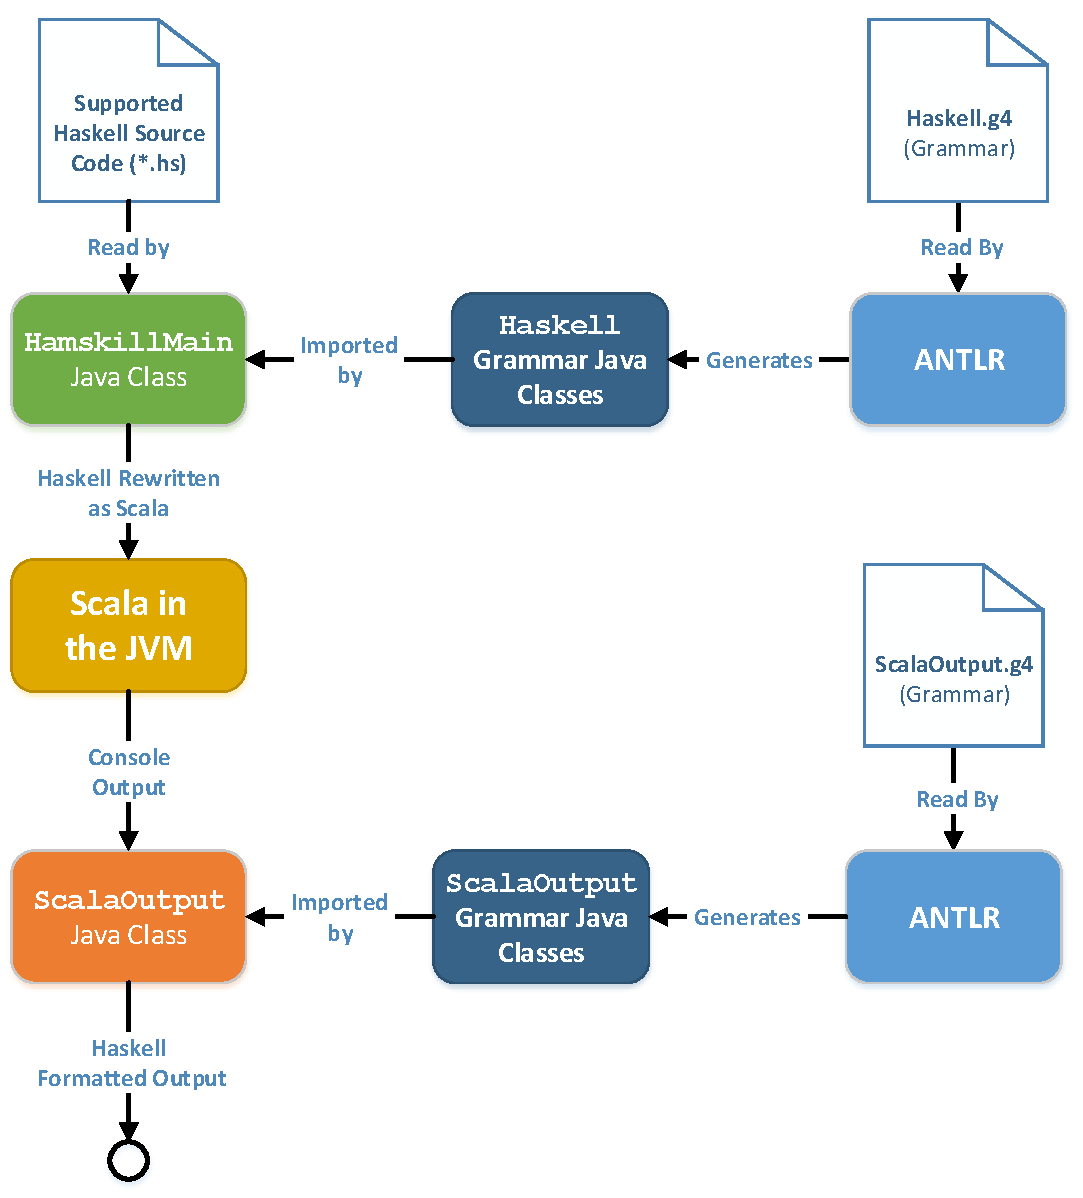
\includegraphics[width=1.0\textwidth]{images/cs252_project_diagram_cropped.pdf}
	\caption{HamSkill Project Architecture}
\end{figure}\label{fig:hamskillArchitecture}

The following subsections describe each of the architecture's components.

\subsection{ANTLR}

ANTLR (\underline{AN}other \underline{T}ool for \underline{L}anguage \underline{R}ecognition) is an adaptive left-to-right, left-most deriviation (LL(*)) lexer and parser written in the Java programming language.  ANTLR's primary function is to read, parse, and process structured text (e.g. Haskell code) \cite{antlrDefinitiveReference}.  

\subsubsection{ANTLR Version 4 Grammar}

A grammar is a formal description of language; it is based off the concept of a context-free grammar in formal automata theory.  ANTLR version 4's (v4) grammar files (denoted by the file extension \emph{.g4}) explicitly define how ANTLR will parse the structured text.  The grammar file may contain token definitions (which always start with a capital letter) and/or parser rules (which always start with a lowercase letter).  A token is a group of characters that form a single object; the parser uses these tokens to recognize sentence structure within a document.

This project utilizes two separate grammars namely: \texttt{Haskell} and \texttt{ScalaOutput}.  They are described in the following two subsections.

\myparagraph{\texttt{Haskell} Grammar}\label{sec:haskellG4}

The \texttt{Haskell} parsing grammar is stored in a file named ``\texttt{Haskell.g4}."  This grammar defines both the tokens and abstract syntax tree for supported Haskell code.  Some of Haskell language features that are supported by this grammar include:

\begin{itemize}
   \item \texttt{case} Statements
   \item \texttt{if}, \texttt{then}, \texttt{else} Conditionals
   \item \texttt{Maybe} Monads
   \item Currying
   \item Partially Applied Functions
   \item Higher Order Functions
   \item Lazy Evaluation
\end{itemize}

For the complete feature set as well as specific Haskell syntax requirements, see section~\ref{sec:hamskillFeatures}.

\myparagraph{\texttt{ScalaOutput} Grammar} 

As mentioned in section~\ref{sec:keyProjectRequirements}, one of the key requirements of this project was that the outputs from Haskell and \textit{HamSkill} be identical.  Figure~\ref{fig:printListHaskell} and~\ref{fig:printListScala} show the Haskell and Scala code respectively to print a list containing integers ``2", ``3", and ``4".  Note that the subsequent lines, which show each language's respective console outputs, are very different.

\begin{figure}[H]
\begin{mdframed}
\begin{lstlisting}[language=Haskell]
Prelude> putStrLn $ show [2, 3, 4]
[2,3,4]
\end{lstlisting}
\end{mdframed}
\caption{Printing a Three Element List in Haskell}\label{fig:printListHaskell}
\end{figure}

\begin{figure}[H]
\begin{mdframed}
\begin{lstlisting}[language=Scala]
scala> println(List(2,3,4))
List(2, 3, 4)
\end{lstlisting}
\end{mdframed}
\caption{Printing a Three Element List in Scala}\label{fig:printListScala}
\end{figure}

The \texttt{ScalaOutput} grammar (contained in the file ``\texttt{ScalaOutput.g4}") corrects these types of differences by parsing the console output of the Scala program and converting that output to a syntax that is more similar to that of Haskell.

\subsubsection{ANTLR Classes}

Programs that use ANTLR do not generally operate directly on the grammar.  Rather, the grammar is converted by ANTLR into a set of Java classes; given an  grammar (e.g. \emph{GrammarName.g4}),  ANTLR would create the following files:

\begin{itemize}
	\item \emph{GrammarName}Lexer.java - This class is the the lexer defined by the input grammar file.  It also extends ANTLR's base \texttt{Lexer} class.
	
	\item \emph{GrammarName}Parser.java - Each rule in the original grammar constitutes a method in this class; it forms the parser class definition associated with the input grammar file.
	
	\item \emph{GrammarName}.tokens - Assigns a token type (e.g. integer, identifier, floating point number etc.) to each token in the input grammar file.
	
	\item \emph{GrammarName}Listener.java \& \emph{GrammarName}BaseListener.java - ANTLR applies the grammar to a text input to build an Abstract Syntax Tree (AST).  While walking the tree, ANTLR fires events that can be captured by a listener\cite{antlrDefinitiveReference}.
	
\end{itemize}

Most programs that want to use ANTLR override the functions in the file \emph{GrammarName}BaseListener.java.


\myparagraph{\texttt{HaskellTokensToScala}}

The class ``\texttt{HaskellTokensToScala}" overrides some of the methods ANTLR auto-generated in the file ``\texttt{HaskellBaseListener.java}"; note that all of these methods are derived from the grammar ``\texttt{Haskell.g4}" described in section~\ref{sec:haskellG4}.  Note that it is the Java code in this file that performs the actual transpilation from Haskell to Scala.

\myparagraph{\texttt{ScalaOutputTokensToHaskellFormat}}\label{sec:scalaOutputFunctionality}

Similar to the \texttt{HaskellTokensToScala} class, the class, ``\texttt{ScalaOutput}" extends the ANTLR auto-generated class, ``\texttt{ScalaOutputBaseListener}".

The listeners in this class are primarily responsible for transforming two different categories of Scala outputs, specifically:

\begin{itemize}

\item \textbf{Lists} - As shown in figures~\ref{fig:printListHaskell} and~\ref{fig:printListScala}, the console output of lists in Scala and Haskell are significantly different.  The methods in this class coupled with the \texttt{ScalaOutput} grammar convert printed lists from Scala to Haskell format.

\item \textbf{\texttt{Maybe}} Monad - The Scala equivalent of Haskell's \texttt{Maybe} monad is named \texttt{Option}.  While the syntax for the two are similar, they are not identical.  For example, ``\texttt{Just}" and ``\texttt{Nothing}" in Haskell are referred to as ``\texttt{Some}" and ``\texttt{None}" in Scala.  The naming convention conversion for console outputs from Scala back to Haskell to is handled by this class.

\end{itemize}

Any other Scala console outputs that do not fall into these two categories are passed through unchanged.


\subsection{Transpiler Output Language: Scala}

As mentioned previously, a transpiler takes source code from one programming language and converts it to code in another language.  It was also previous explained that the primary criteria when deciding on the output language was that it needed to be runnable in the Java Virtual Machine.  Other important criteria that guided language selection were:

\begin{itemize}

	\item \textbf{Higher Order Function Support} - Any language that is devoid of higher order support would be a poor match for a purely functional language like Haskell.
	
	\item \textbf{Similar Syntactic Structure} - Closer alignment between the input and output languages will simplify the transcompilation.  Inevitably though, some amount of restructuring and reformatting will be required.  
	
	\item \textbf{Personal Interest} - Increased personal investment in a project topic generally leads to a more fulfilling outcome for the student and a better project overall.  

\end{itemize}

The language that best fit these criteria is Scala, which is a functional language which can be fully run inside the JVM \cite{whatIsScala}. What is more, Scala natively supports many of Haskell's core features including: functions written in a pattern matching style, immutability of objects, currying, partially applied functions, lazy evaluation, static typing, etc.  One of the disadvantages of Scala is its weaker type inference in comparison to Haskell; due to this, specific requirements were placed on the Haskell dialect supported by \textit{HamSkill} as described in section \ref{sec:hamskillFeatures}.  It is also important to note that the author has had a personal predisposed interest to learning Scala given its extensive support by Apache Spark.  Given all of these factors, the selection of Scala for this project became an even more obvious choice.

\textit{HamSkill} implements two different schemes for running the transpiled Scala code, namely \textit{HamSkill} Standard and \textit{HamSkill}+.  They are described in the follow subsections.

\myparagraph{\textit{HamSkill} Standard}

Since Scala is a compiled language, it does not lend itself tremendously well to Java runtime compilation and execution.  To workaround this, I leveraged Twitter's \texttt{util-eval} library, which allows runtime compilation and execution of Scala code entirely within a Java program \cite{githubTwitterEvalUtil}.  The advantages and disadvantages of using  this library are:

\begin{itemize}

\item \textbf{Advantages}:

\begin{enumerate}

\item \textbf{Reduced JVM Requirements} - Twitter's \texttt{util-eval} library is a JAR file that only requires the presence of Scala's compile and main library JAR files to run.  Hence, this eliminates the need for the user to have Scala installed in their environment.  This addresses one of the key requirements enumerated in section~\ref{sec:keyProjectRequirements}.

\item \textbf{Simplified Usage} - When \textit{HamSkill} Standard is used, the number of steps the system must perform to transpile, compile, then run the Scala code is non-trivial.  A single call to \textit{HamSkill} standard's main function performs all three of these steps.  In contrast, \textit{HamSkill}+ requires at least three steps to do the same task introduction additional possible points of failure..

\end{enumerate}

\item \textbf{Disadvantages}:

\begin{enumerate}

\item \textbf{Reduced Feature Set} - The \texttt{util-eval} library does not support all Scala features.  An example of a missing feature is \texttt{readLine} which takes console inputs.

\item \textbf{Reliance on Third Party Developers} - As mentioned previously, \texttt{util-eval} was developed by Twitter.  Hence, it can be deprecated at any time as was previously planned \cite{deprecateUtilEval}.  While the tool is open-source, picking up a dropped project introduces an additional set of complications.

\end{enumerate}

\end{itemize}

\myparagraph{\textit{HamSkill}+}

Unlike \textit{HamSkill} Standard, \textit{HamSkill}+ requires Scala to be installed on the host PC.  What this then enables is that any feature that is supported by the install version of Scala could in theory be supported by \textit{HamSkill}+.  Currently, running a Haskell program in \textit{HamSkill}+ requires four separate steps, all of which are controlled by a \texttt{bash} scripts as shown in figures~\ref{fig:runHamskill},~\ref{fig:compileScala}, and~\ref{fig:runScalaAndConvertOutput}.

\begin{enumerate}

\item \textbf{Transpile the Haskell code to Scala} - This is done by running the \texttt{main} method in the \texttt{HamskillMain} class as shown in figure~\ref{fig:runHamskill}.  Note that ``\texttt{"\$@"}" in \texttt{bash} means that any parameters passed to the \texttt{bash} script are directly passed as arguments into the \texttt{main} method.  In \textit{HamSkill+}, the last argument is the name of the file where the Scala code will be written.

\begin{figure}[H]
\begin{mdframed}
\begin{lstlisting}[language=bash]
java -jar hamskill.jar "$@"
\end{lstlisting}
\end{mdframed}
\caption{Executing the Transpilation for \texttt{HamSkill}+}\label{fig:runHamskill}
\end{figure}

\item \textbf{Compile the Transpiled Scala Code} - The \texttt{bash} command to compile Scala is ``\texttt{scalac}" as shown in figure~\ref{fig:compileScala}.  Note that ``\texttt{\$scalaSrcFile}" is the filename where the transpiled Scala code was written.

\begin{figure}[H]
\begin{mdframed}
\begin{lstlisting}[language=bash]
scalac $scalaSrcFile
\end{lstlisting}
\end{mdframed}
\caption{Executing the Transpiled Code in \texttt{HamSkill}+}\label{fig:compileScala}
\end{figure}

\item \textbf{Execute the Transpiled Scala Code} - The \texttt{bash} command to run a compiled Scala class is simply ``\texttt{scala}" as shown in figure~\ref{fig:runScalaAndConvertOutput}.  Note that ``\texttt{\$scalaSrcFile}" is the filename where the transpiled Scala code was written.

\begin{figure}[H]
\begin{mdframed}
\begin{lstlisting}[language=bash]
scala -cp . $scalaObject 
          | java -cp hamskill.jar hamskill.ScalaOutput
\end{lstlisting}
\end{mdframed}
\caption{Executing the Scala Code and Piping to \texttt{ScalaOutput}}\label{fig:runScalaAndConvertOutput}
\end{figure}

\item \textbf{Pipe Scala Output to the \texttt{ScalaOutput} Class} - The console output of the Scala code is piped (``\texttt{|}") into the standard Java class \texttt{ScalaOutput} as shown in figure~\ref{fig:runScalaAndConvertOutput}.  As explained in section~\ref{sec:scalaOutputFunctionality}, this class performs any necessary transformations on the console outputs and then prints them to the console as if the original code had been run in Haskell.

\end{enumerate} 

\section{Haskell Features Supported by \textit{HamSkill}}\label{sec:hamskillFeatures}

This section enumerates the Haskell features that are supported by \textit{HamSkill}.  It also enumerates any specific formatting requirements for the \textit{HamSkill} Haskell dialect.

\subsection{Single Haskell File}

Currently, \textit{HamSkill} only supports a single Haskell file at a time.  If the user wanted to support code across multiple files, s/he could transpile the code to Scala, manually configure the imports, and then run the Scala code manually.  While this requirement may be a bit onerous, it should not detract limit the tool's overall capabilities in a substantial way.

\subsection{Functions}

Functions written in Haskell can be interpretted by \textit{HamSkill}.  Figure~\ref{fig:myFunctionHaskell} is a function from the \textit{HamSkill} testcase named ``\texttt{simple\_function\_call.hs}".

\begin{figure}[H]
\begin{mdframed}
\begin{lstlisting}[language=Haskell]
myFunc :: [Int] -> Int -> Int
myFunc x y = 3 + 5
\end{lstlisting}
\end{mdframed}
\caption{Simple \textit{HamSkill} Function}\label{fig:myFunctionHaskell}
\end{figure}

The following subsections enumerate the requirements a Haskell function must satisfy to be supported by \textit{HamSkill}.

\subsubsection{Valid Function Prototype}

All functions (excluding partially applied functions described in section~\ref{sec:partiallyAppliedFunctions}) must have a valid function prototype.  Note that only a subset of Haskell's base classes are supported (see section \ref{sec:supportedTypes} for the list).  Note that type variables (even if they map to a supported type) are not supported.

\subsubsection{Pattern Matching}\label{sec:supportedPatternMatching}

As shown in figure~\ref{fig:myFuncDefinition}, pattern matching of function variables is supported.  Special pattern matching cases that HamSkill can handle include:

\begin{itemize}

\item Ignored variables via Underscore(\texttt{\_})

\item Prepend using Colon (\texttt{:})

\item Empty List (\texttt{[ ]})

\end{itemize}

Figure~\ref{fig:functionZaydFoldr} is a function from the \textit{HamSkill} test case ``" that uses three of the four the previously mentioned special pattern matching cases.

\begin{tiny}
\begin{figure}[H]
\begin{mdframed}
\begin{lstlisting}[basicstyle=\small, language=Haskell]
zayd_foldr :: (Int -> Int -> Int) -> Int -> [Int] -> Int
zayd_foldr _ acc [] = acc
zayd_foldr f acc (x:xs) = f (x) (zayd_foldr (f) (acc) (xs))
\end{lstlisting}
\end{mdframed}
\caption{\textit{HamSkill} Pattern Matching Example}\label{fig:functionZaydFoldr}
\end{figure}
\end{tiny}

Note that guards are not currently supported.

\subsubsection{A Single Executable Command per Pattern Matching Case}

For each pattern matching case, only a single command is allowed; Haskell's \texttt{where} and \texttt{let} syntaxes are not supported.  For example, note that for the single pattern matching case in the function ``\texttt{myFunc}" in figure~\ref{} only executes a single command (i.e. ``\texttt{3 + 5}").

If the user wants to define subvariables or execute multiple commands for a single pattern matching case, these additional steps must be defined as separate functions.  While this requirement may make a developer's code more verbose, it should limit the capabilities of the user.

\subsubsection{Recursion}

Recursion is supported by \textit{HamSkill}; however, there are requirements on how function function parameters must be specified as explained in section~\ref{sec:nestedFunctionCalls}.

Figures~\ref{fig:functionZaydFoldr} and~\ref{fig:functionAddList} are recursive functions supported by \textit{HamSkill}; note that the function in figure~\ref{fig:functionAddList} is in the \textit{HamSkill} test case named ``\texttt{addList.hs}".

\begin{tiny}
\begin{figure}[H]
\begin{mdframed}
\begin{lstlisting}[language=Haskell]
addList :: [Int] -> Int
addList [] = 0
addList (x:xs) = x + (((addList xs)))
\end{lstlisting}
\end{mdframed}
\caption{Recursive Haskell Function to Add All Integers in a List}\label{fig:functionAddList}
\end{figure}
\end{tiny}

\subsubsection{Empty Line at the End of the File}

After the last function in the file, there must be at least a single empty line.  This requirement was included because it simplifies the parsing process.

\subsection{\texttt{main} Function}

Every Haskell file that is run in either \textit{HamSkill} Standard or \textit{HamSkill}+ must have a \texttt{main} function.  This function is sole entry point into the HamSkill function.  As with all functions, this method must have a function prototype.

Unlike other functions, multiple distinct statements may appear in the main block; these statements may even use the syntax ``\texttt{<-}" as long as they are being used to unbox a Haskell \texttt{IO String} object.

Figure~\ref{fig:functionHaskellMainConsoleInput} is a recursive, multi-instruction \texttt{main} function that supports taking text inputs from the console, and then prints them to the screen.  This figure also shows the special syntax required when recursing on main where the function name must be surrounded by triple parentheses (i.e. ``\texttt{(((main)))}").  This was done to simplify the parsing to let HamSkill know that this is a recursive call and that when converting this code to Scala, it must pass it an argument as shown in figure~\ref{fig:functionScalaMainConsoleInput}; this \texttt{main} recursive syntax is only supported within the \texttt{main} method itself.

\begin{tiny}
\begin{figure}[H]
\begin{mdframed}
\begin{lstlisting}[language=Haskell]
main :: IO ()
main = do 
     x <- getLine 
     putStrLn $ x
     if (length x == 0) 
     then 
          (return () )
     else
          ( (((main))) )
\end{lstlisting}
\end{mdframed}
\caption{Haskell Function That Takes and Prints Console Inputs}\label{fig:functionHaskellMainConsoleInput}
\end{figure}
\end{tiny}

\begin{tiny}
\begin{figure}[H]
\begin{mdframed}
\begin{lstlisting}[language=scala]
  def main(args : Array[String]){
    lazy val x = scala.io.StdIn.readLine();
     println (x)
     if((x).length() == 0)
      {
         return;
      }
      else{
         main(args)
      }
  } // End of function
\end{lstlisting}
\end{mdframed}
\caption{\textit{HamSkill} Generated Scala Code to Take and Print Console Inputs}\label{fig:functionScalaMainConsoleInput}
\end{figure}
\end{tiny}

Note that the code shown in figure~\ref{fig:} is only supported in \textit{HamSkill}+.

\subsection{Currying}\label{sec:currying}

Haskell is a fully curried language \cite{learnYouAHaskell}.  In contrast, a Scala function's prototype must be specially formatted to support currying by default. Figure~\ref{fig:myFuncInScalaNoCurrying} shows Scala code generated by \textit{HamSkill} with currying disabled (note the Haskell version of ``\texttt{myFunc}" is shown figure~\ref{fig:myFunctionHaskell}); in contrast, figure~\ref{fig:myFuncInScalaWithCurrying} shows the \textit{HamSkill} generated Scala code with currying enabled.  Notice that when currying is enabled, each of the function parameter is inside its own set of parentheses.

\begin{tiny}
\begin{figure}[H]
\begin{mdframed}
\begin{lstlisting}[basicstyle=\small, language=scala]
  def myFunc(___0___ : => Array[Int], ___1___ : => Int) : 
                           Int = (___0___, ___1___) match {
      case (x, y) => 3 + 5
  } 
\end{lstlisting}
\end{mdframed}
\caption{\textit{HamSkill} Generated Scala Code for Function \texttt{myFunc} with \textbf{No} Currying}\label{fig:myFuncInScalaNoCurrying}
\end{figure}
\end{tiny}

\begin{tiny}
\begin{figure}[H]
\begin{mdframed}
\begin{lstlisting}[basicstyle=\small, language=scala]
  def myFunc(___0___ : => Array[Int], ___1___ : => Int) : Int = (___0___, ___1___) match {
      case (x, y) => 3 + 5
  } 
\end{lstlisting}
\end{mdframed}
\caption{\textit{HamSkill} Generated Scala Code for Function \texttt{myFunc} \textbf{with} Currying}\label{fig:myFuncInScalaWithCurrying}
\end{figure}
\end{tiny}  

\subsection{Supported Types}\label{sec:supportedTypes}

\emph{HamSkill} only supports a select subset of Haskell's available types, namely: \texttt{Bool}, \texttt{\tt Integer} (i.e. bounded), and finite \texttt{List}s.

While implementing floating point numbers would not add substantial complexity at a basic level, ensuring that the floating point behavior of \emph{HamSkill} (i.e. Scala) and Haskell are identical is beyond the scope of this project.

\subsection{Immutability in Scala}\label{sec:immutabilityScala}

One of the key features of Haskell that allows it to achieve referential transparency is the immutability of data.  While it would be possible to develop an infrastructure in a language like Python to assure immutability, it is an encumbrance.  In cases such as this, it is almost always better to take advantage of a language's native features when possible.  In Scala, the {\tt val} construct ensure the immutability of an object without any user intervention.  For example, the code in figure~\ref{fig:scalaValConstruct} would raise a runtime error since it is trying to change the value of immutable data.

\begin{figure}[H]
\begin{mdframed}
\begin{lstlisting}[language=Scala]
val x = 5
x = 3
\end{lstlisting}
\end{mdframed}
\caption{Declaring Immutable Data in Scala}\label{fig:scalaValConstruct}
\end{figure}

\subsection{Lazy Evaluation}\label{sec:lazyEvaluationScala}

Another important aspect of Haskell is that it supports lazy evaluation.  This entails that data's value is not calculated until it is not needed.  Figure \ref{fig:lazyImmutabilityInScala} is an example of lazy evaluation with Scala as when this code is run, it will print a negative elapsed time (which is clearly not correct).

\begin{figure}[H]
\begin{mdframed}
\begin{lstlisting}[language=Scala]
def lazyTime(){
  lazy val t1 = System.nanoTime()
  val t2 = System.nanoTime()
  Thread.sleep(1000)
  println("Elapsed time is " + (t2-t1)/1000000 + "ms")
}
\end{lstlisting}
\end{mdframed}
\caption{Lazy, Immutable Code in Scala}\label{fig:lazyImmutabilityInScala}
\end{figure}

Scala also supports ``call-by-name" to achieve laziness of function parameters.  However, this feature is not truly lazy as it will recalculate the value each time the parameter is used in the function.  This limitation often degrades the overall the performance; for this reason, I do not plan to implement laziness in \emph{HamSkill} across functions.



\subsection{Conversion from Functions to Methods}

The function in Haskell to convert data to string is ``{\tt show}". In contrast, the syntax in Scala to convert an object (e.g. ``x") to a string is ``{\tt x.toString()}".  Due to this, the ANTLR parser will need to be able to convert a prefix function to an object method call.

\subsection{Nested Function Calls}\label{sec:nestedFunctionCalls}

Imperative languages (e.g. Java) are generally more verbose than functional languages; Haskell is no exception to this.  Conciseness introduces significant challenges when writing a parser as the contextual information is reduced.  For example, figure \ref{fig:addTwoNumbersHaskell} is a simple line of Haskell code that prints to the screen the result of a function ``{\tt addTwoNumbs}" that takes two integers (e.g. ``{\tt x}" and ``{\tt y}") and sums them. 

\begin{figure}[H]
\begin{mdframed}
\begin{lstlisting}[language=Haskell]
putStrLn $ show $ addTwoNumbs x y
\end{lstlisting}
\end{mdframed}
\caption{Simple Function Call in \textbf{Haskell}}\label{fig:addTwoNumbersHaskell}
\end{figure}

Similar code in Java is shown in figure \ref{fig:addTwoNumbersJava}

\begin{figure}[H]
\begin{mdframed}
\begin{lstlisting}[language=Java]
System.out.println( addTwoNumbs(x, y) ) ;
\end{lstlisting}
\end{mdframed}
\caption{Simple Function Call in \textbf{Java}}\label{fig:addTwoNumbersJava}
\end{figure}

The Java syntax explicitly shows that {\tt addTwoInts} is a function since the parameters are inside parentheses and are comma separated.  To simplify the parsing for this in Haskell, the \emph{HamSkill} requires function arguments to be preceded and succeeded by triple parentheses ``\texttt{(((}" and ``\texttt{)))}".  Figure \ref{fig:addTwoNumbersHamSkill} shows the \emph{HamSkill} version of the Haskell code in figure \ref{fig:addTwoNumbersHamSkill}.

\begin{figure}[H]
\begin{mdframed}
\begin{lstlisting}[language=Haskell]
putStrLn $ show $ addTwoInts ((x y))
\end{lstlisting}
\end{mdframed}
\caption{Simple Function Call in \textbf{\emph{HamSkill}}}\label{fig:addTwoNumbersHamSkill}
\end{figure}

\subsection{Defining Scope and Scala Object Name via {\tt module}}

A program in Haskell is composed of a set of ``{\tt module}" files.  The ``{\tt module}" keyword is used to  scope of functions (e.g. {\tt public} or {\tt private}) as well as for defining an abstract data type \cite{haskellModule}.  In \emph{HamSkill}, I will use the Haskell module to define whether the Scala methods are private (since by default functions are {\tt public}) as well as the name of the Scala object.

\subsection{Partially Applied Functions}\label{sec:partiallyAppliedFunctions}

Haskell supports partially applied functions.  Figure \ref{fig:addFiveHaskell} shows the {\tt addTwoInts} function with a single argument (i.e. ``{\tt 5}") being stored in a variable ``{\tt addFive}".  

\begin{figure}[H]
\begin{mdframed}
\begin{lstlisting}[language=Haskell]
let addFive = addTwoInts 5
\end{lstlisting}
\end{mdframed}
\caption{Partially Applied addTwoInts Function in \textbf{Haskell}}\label{fig:addFiveHaskell}
\end{figure}

Partially applied functions in Scala have advantages and disadvantages in comparison to Haskell.  One of these disadvantages is evident when figures \ref{fig:addFiveHaskell} and \ref{fig:addFiveScala} are compared.  Note that the Scala function requires an underscore ("\_") for each missing argument as well as the type for that argument.  This makes converting Haskell code to Scala problematic as the function prototype must be fixed and known at conversion time.  

\begin{figure}[H]
\begin{mdframed}
\begin{lstlisting}[language=Scala]
val addFive = addTwoInts(5, _: Int)
\end{lstlisting}
\end{mdframed}
\caption{Partially Applied {\tt addTwoInts} Function in \textbf{Scala}}\label{fig:addFiveScala}
\end{figure}

To simplify this, \emph{HamSkill} will require that any partially defined functions are declared in the same file/module.  I will investigate using a predefined list of functions, but this may not be feasible or support will be very limited due to the requirement to define the parameter type.  What is more, partially applied functions will use need to use the ``triple parentheses style" described in section \ref{sec:nestedFunctionCalls}.

\subsection{Higher Order Function Support}\label{sec:higherOrderFunctions}

Scala and Haskell are both functional programming languages; one important consequence of this is that both support higher order functions.  \emph{HamSkill} will support functions as input parameters to functions.  If time allows, I will also investigate the ability to return functions from functions.  The extent to which this is supported will be dependent on the extent to which partially applied functions are supported as defined in section \ref{partiallyAppliedFunctions}.

\subsection{Haskell Lambda Function to Scala Anonymous Functions}\label{sec:lambdaAnonymousFunctions}

There is significant similarity between a Lamda function in Haskell and an anonymous function in Scala.  One primary difference is that Scala requires the developer to specify the types of the parameters in the anonymous function while Scala does not. For this project, I will implement support for anonymous functions either as parameters to other functions or for support for an operation such as folding or filtering a list. 

\subsection{Maybe Monad Support}

\subsection{Preserving Comments}\label{sec:preservingComments}

\section{\textit{HamSkill} Testing Overview}

Software testing is important for detecting defects in software programs.  What is more, there is different types of software testing including unit testing, module level testing, and system tests.  Given that ANTLR relies heavily on the Listener pattern, it reduces the ease at which unit testing can be performed.  What is more, given that \textit{HamSkill} relies on the end to end operation of programs written in Haskell, ANTLR, Java, and Scala, it really emphasizes the importance of system level test.

\subsection{System Level and Regression Testing}

\textit{HamSkill}'s uses black-box system level testing.  A set of use cases (i.e. Haskell files) were generated by me; these files are then run through both Haskell (to verify they are valid Haskell code) and through \textit{HamSkill}; the resulting outputs are then compared.  If the outputs are the same, the test is considered successful; in the case of any difference, the test is classified as a failure.  The full set of \textit{HamSkill} test cases are included with this submission in the folder \path{Test_Bench/test_cases}.

Regression testing verifies that new features do not affect/compromise existing ones.  When developing HamSkill, I iteratively added new features.  After each feature was added, I reran the entire test bench to ensure that no new (detectable) issues were introduced.  If an issue did arise, I would immediately address before moving on to new features to ensure that fundamental problems did not compound upon themselves. This formed a type of regression testing throughout my development.

\subsection{Test Bench Implementation Overview}

The \textit{HamSkill} test architecture is written as a \texttt{bash} script (see the file in the submission \path{Test_Bench/test_bench.sh}.  The function ``\path{perform_hamskillStd_and_hamskillPlus_test}" is the most important in the script as it is used to perform most of the testing; the basic operational flow of this function is:

\begin{itemize}

\item \textbf{Step \#1}: The function is provided the name of a Haskell program written in the dialect supported by \textit{HamSkill}, but without the file extension.

\item \textbf{Step \#2}: The Haskell program is run in Haskell, and the program's output is stored to a specific file on disk using the \texttt{bash} command ``\texttt{>}". 

\item\label{item:runHamSkillStandard} \textbf{Step \#3}: Run HamSkill in standard mode and store the results to a file using the bash command ``\texttt{>}". 

\item\label{item:diffHamSkillStandard} \textbf{Step \#4}: Perform a file difference operation (using the \texttt{bash} \texttt{diff} command) on the output files from Haskell and HamSkill standard.  If the two files are identical, then mark the test as passing; if they are different, the test fails.
 
\item \textbf{Step \#5}: Repeat steps \#~\ref{item:runHamSkillStandard} and \#~\ref{item:diffHamSkillStandard} using \texttt{HamSkill+}.

\end{itemize}

There is an additional function in the \texttt{bash} test bench named ``\texttt{print\_final\_results}" that prints the final results (i.e. number of passing tests versus the total number of tests).

\section{Conclusions}

\textit{HamSkill} provides a foundation for running a dialect of Haskell inside the JVM.  All of the original key features outlined in the proposal were implemented as well as additional features including Monads and the Scala output reformatter.  While \textit{HamSkill} does have limitation as all languages do (in particular those with a scope as limited as this), it is viewed by the development team as a very successful project that has exceeded our expectations.

\pagebreak
\bibliographystyle{plainurl}
\bibliography{final_report_biblio}

\end{document}
